\documentclass[12pt]{article}
\usepackage{fullpage,enumitem,amsmath,amssymb,graphicx,grffile,float,listings}



\begin{document}
    %Title Section
    \begin{flushleft}
    \LARGE CS229 Fall 2017\\
    \LARGE Problem Set \#2:  Supervised Learning II    \\
    \textbf{\normalsize Author: LFhase \quad rimemosa@163.com}
    \end{flushleft} 
    \noindent
    \rule{\linewidth}{0.4pt}
    %Title Section

    %Problem and Solution

    \section*{Logistic Regression: Training stability  }

    \begin{enumerate}[label=(\alph*)]
    \item Training model on dataset A costs far more less time than that on dataset B, which means that training on dataset B does't converge.
    \item 
    Let's plot the training results after 10000, 20000, 30000, 40000 iterations.
    \begin{figure}[H]
        \centering
        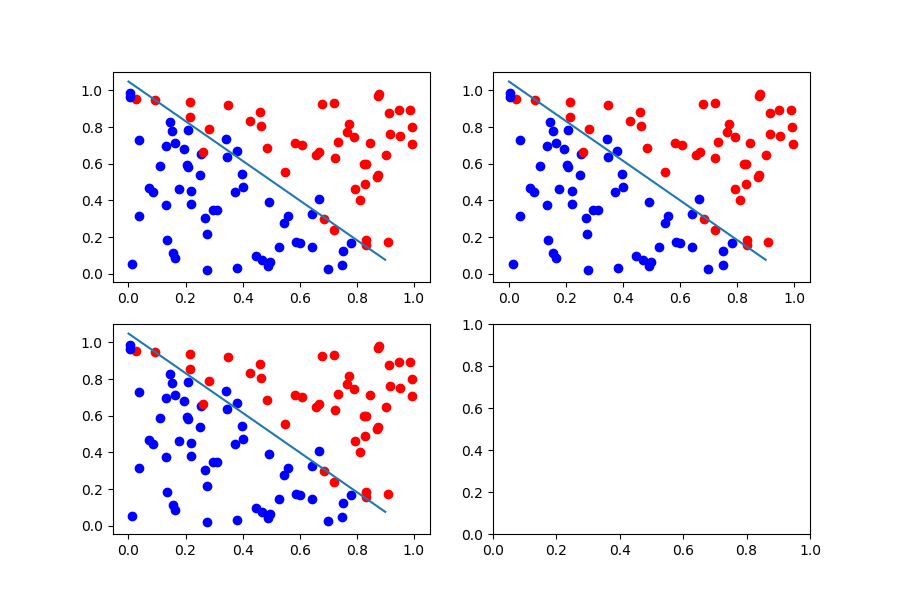
\includegraphics[width=0.80\textwidth]{Q1/training_dsA.png}
        \caption{Training Results on Dataset A}
    \end{figure}
    \begin{figure}[H]
        \centering
        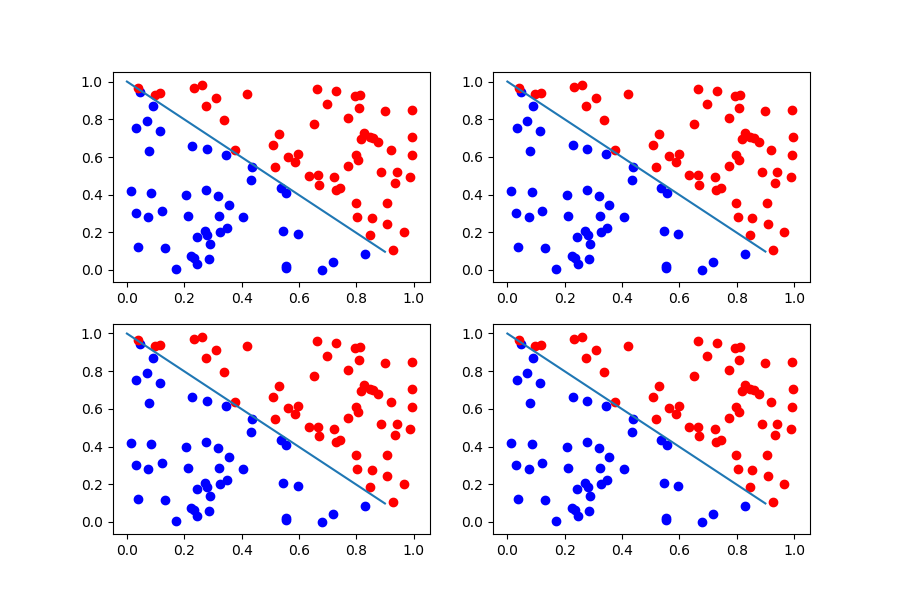
\includegraphics[width=0.80\textwidth]{Q1/training_dsB.png}
        \caption{Training Results on Dataset B}
    \end{figure}
    From the above two figures, we can see that data on dataset B is hardly to separate (Bad Linearly Separability), which may be the main issue resluting nonconvergence.
    \item 
    \begin{enumerate}[label=\roman*]
        \item No. Using a different learning rate only changes the learning speed here, but it won't change the fact that the algorithm has to find the hyperline in hardly separable data.
        \item No. The same to the former.
        \item Yes. It will stop $||\theta||$ being infinitely large.
        \item No. It doesn't change the linearly separability.
        \item Yes. It will expand the feature space, which may let the data linearly separable.
    \end{enumerate}
    \item Yes. It will put the data into a new feature space, where the data may become linearly separable.
    \end{enumerate}

    \newpage
    \section*{Model Calibration}
    \begin{enumerate}[label=(\alph*)]
    \item gg
    \end{enumerate}
\end{document}